\documentclass[12pt,a4paper,bibliography=totocnumbered,listof=totocnumbered]{scrartcl}
\usepackage[ngerman]{babel}
\usepackage[utf8]{inputenc}
\usepackage{amsmath}
\usepackage{amsfonts}
\usepackage{amssymb}
\usepackage{graphicx}
\usepackage{fancyhdr}
\usepackage{tabularx}
\usepackage{geometry}
\usepackage{setspace}
\usepackage[right]{eurosym}
\usepackage[printonlyused]{acronym}
\usepackage{subfig}
\usepackage{floatflt}
\usepackage[usenames,dvipsnames]{color}
\usepackage{colortbl}
\usepackage{paralist}
\usepackage{array}
\usepackage{titlesec}
\usepackage{parskip}
\usepackage[right]{eurosym}

\usepackage[subfigure,titles]{tocloft}
\usepackage[pdfpagelabels=true]{hyperref}

\usepackage{listings}
\lstset{basicstyle=\footnotesize, captionpos=b, breaklines=true, showstringspaces=false, tabsize=2, frame=lines, numbers=left, numberstyle=\tiny, xleftmargin=2em, framexleftmargin=2em}
\makeatletter
\def\l@lstlisting#1#2{\@dottedtocline{1}{0em}{1em}{\hspace{1,5em} Lst. #1}{#2}}
\makeatother

\geometry{a4paper, top=27mm, left=30mm, right=20mm, bottom=35mm, headsep=10mm, footskip=12mm}

\hypersetup{unicode=false, pdftoolbar=true, pdfmenubar=true, pdffitwindow=false, pdfstartview={FitH},
	pdftitle={Fallstudie GIT},
	pdfauthor={Vedad Hamamdzic},
	pdfsubject={Abschlussarbeit},
	pdfcreator={\LaTeX\ with package \flqq hyperref\frqq},
	pdfproducer={pdfTeX \the\pdftexversion.\pdftexrevision},
	pdfkeywords={Ausarbeitung},
	pdfnewwindow=true,
	colorlinks=true,linkcolor=black,citecolor=black,filecolor=magenta,urlcolor=black}
\pdfinfo{/CreationDate (D:20110620133321)}

\begin{document}

\titlespacing{\section}{0pt}{12pt plus 4pt minus 2pt}{-6pt plus 2pt minus 2pt}

% Kopf- und Fusszeile
\renewcommand{\sectionmark}[1]{\markright{#1}}
\renewcommand{\leftmark}{\rightmark}
\pagestyle{fancy}
\lhead{}
\chead{}
\rhead{\thesection\space\contentsname}
\lfoot{Fallstudie Entwicklungswerkzeuge: GIT\newline}
\cfoot{}
\rfoot{\ \linebreak Seite \thepage}
\renewcommand{\headrulewidth}{0.4pt}
\renewcommand{\footrulewidth}{0.4pt}

% Vorspann
\renewcommand{\thesection}{\Roman{section}}
\renewcommand{\theHsection}{\Roman{section}}
\pagenumbering{Roman}

% ----------------------------------------------------------------------------------------------------------
% Titelseite
% ----------------------------------------------------------------------------------------------------------
\thispagestyle{empty}
\begin{center}
	
\includegraphics[scale=1]{Bilder/hs_os.png}\\
	\vspace*{2cm}
	\Large
	\textbf{Fallstudie Entwicklungswerkzeuge}\\
	\textbf{}\\
	\vspace*{2cm}
	\Huge
	\textbf{Ausarbeitung}\\
	\vspace*{0.5cm}
	\large
	über das Thema\\
	\vspace*{1cm}
	\textbf{GIT Versionsverwaltungssystem}\\
	\vspace*{2cm}
	
	\vfill
	\normalsize
	\newcolumntype{x}[1]{>{\raggedleft\arraybackslash\hspace{0pt}}p{#1}}
	\begin{tabular}{x{6cm}p{7.5cm}}
		\rule{0mm}{5ex}\textbf{Autor:} & Vedad Hamamdzic\newline email@email.de \\ 
		\rule{0mm}{5ex}\textbf{Prüfer:} & Paul Layer \\ 
		\rule{0mm}{5ex}\textbf{Abgabedatum:} & 18.11.2014 \\ 
	\end{tabular} 
\end{center}
\pagebreak

% ----------------------------------------------------------------------------------------------------------
% Abstract
% ----------------------------------------------------------------------------------------------------------
\setcounter{page}{1}
\onehalfspacing
\titlespacing{\section}{0pt}{12pt plus 4pt minus 2pt}{2pt plus 2pt minus 2pt}
\rhead{KURZFASSUNG}
\section{Zusammenfassung}

Lorem ipsum dolor sit amet, consetetur sadipscing elitr, sed diam nonumy eirmod tempor invidunt ut labore et dolore magna aliquyam erat, sed diam voluptua. At vero eos et accusam et justo duo dolores et ea rebum. Stet clita kasd gubergren, no sea takimata sanctus est Lorem ipsum dolor sit amet. Lorem ipsum dolor sit amet, consetetur sadipscing elitr, sed diam nonumy eirmod tempor invidunt ut labore et dolore magna aliquyam erat, sed diam voluptua. At vero eos et accusam et justo duo dolores et ea rebum. Stet clita kasd gubergren, no sea takimata sanctus est Lorem ipsum dolor sit amet.

\vspace{-1,2em}
\titlespacing{\section}{0pt}{12pt plus 4pt minus 2pt}{-6pt plus 2pt minus 2pt}
\section*{Abstract}
Das ganze auf Englisch.
\pagebreak

% ----------------------------------------------------------------------------------------------------------
% Verzeichnisse
% ----------------------------------------------------------------------------------------------------------
% TODO Typ vor Nummer
\renewcommand{\cfttabpresnum}{Tab. }
\renewcommand{\cftfigpresnum}{Abb. }
\settowidth{\cfttabnumwidth}{Abb. 10\quad}
\settowidth{\cftfignumwidth}{Abb. 10\quad}

\titlespacing{\section}{0pt}{12pt plus 4pt minus 2pt}{2pt plus 2pt minus 2pt}
\singlespacing
\rhead{INHALTSVERZEICHNIS}
\renewcommand{\contentsname}{II Inhaltsverzeichnis}
\phantomsection
\addcontentsline{toc}{section}{\texorpdfstring{II \hspace{0.35em}Inhaltsverzeichnis}{Inhaltsverzeichnis}}
\addtocounter{section}{1}
\tableofcontents
\pagebreak
\rhead{VERZEICHNISSE}
\listoffigures
\pagebreak
\listoftables
%\pagebreak
\renewcommand{\lstlistlistingname}{Listing-Verzeichnis}
{\labelsep2cm\lstlistoflistings}
\pagebreak

% ----------------------------------------------------------------------------------------------------------
% Abkürzungen
% ----------------------------------------------------------------------------------------------------------
\section{Abkürzungsverzeichnis}
\begin{acronym}[OSGi] % längste Abkürzung steht in eckigen Klammern
	\setlength{\itemsep}{-\parsep} % geringerer Zeilenabstand
	\acro{OSGi}{Open Service Gateway initiative}
\end{acronym}
\newpage

% ----------------------------------------------------------------------------------------------------------
% Inhalt
% ----------------------------------------------------------------------------------------------------------
% Abstände Überschrift
\titlespacing{\section}{0pt}{12pt plus 4pt minus 2pt}{-6pt plus 2pt minus 2pt}
\titlespacing{\subsection}{0pt}{12pt plus 4pt minus 2pt}{-6pt plus 2pt minus 2pt}
\titlespacing{\subsubsection}{0pt}{12pt plus 4pt minus 2pt}{-6pt plus 2pt minus 2pt}

% Kopfzeile
\renewcommand{\sectionmark}[1]{\markright{#1}}
\renewcommand{\subsectionmark}[1]{}
\renewcommand{\subsubsectionmark}[1]{}
\lhead{Kapitel \thesection}
\rhead{\rightmark}

\onehalfspacing
\renewcommand{\thesection}{\arabic{section}}
\renewcommand{\theHsection}{\arabic{section}}
\setcounter{section}{0}
\pagenumbering{arabic}
\setcounter{page}{1}

% ----------------------------------------------------------------------------------------------------------
% Einleitung
% ----------------------------------------------------------------------------------------------------------
\section{GIT}

\subsection{Was ist ein Versionskontrollsystem}
GIT ist ein Versionsverwaltungssystem, soviel wissen wir. Doch was ist das und was macht es im Detail? Ein Versionsverwaltungssystem ist ein System, welches Änderungen an einer Datei oder eine Reihe von Dateien protokolliert, so dass  bestimmte Versionen später wieder aufrufbar sind.\footnote{\cite{chacon2009pro} Seite 1 Zeile 1 } Um Problemen entgegenzuwirken die eine amateurhafte Methoden der Versionsverwaltung mit sich bringen, wie z.B das ständige kopieren neuer Versionen in ein Verzeichnis, hierfür wurden diese Systeme entwickelt.Dabei unterscheidet man 3 Arten von Systemen. Der wesentlichste Unterschied, besteht darin wie und wo die Daten gehalten werden.

\subsubsection{Lokale Versionskontrollsysteme}
Von Lokalen Versionskontrollsystemen spricht man, wenn die Daten auf dem Lokalen System vorliegen (siehe Abbildung 1 ). Dabei werden die Dateien in einer Version Database (Repository) gehalten. Nach jedem Checkout wird automatisch eine neue Version im Repository erstellt. Somit entgeht man der Gefahr, durch das oben erwähnte Kopieren in andere Verzeichnisse, eine der Versionen zu überschreiben, da man vergessen hat die Datei umzubenennen. Natürlich ist diese Variante der Versionskontrolle, für große Projekte die im Team bearbeitet werden eher destruktiv. Ein Beispiel für Lokale Systeme ist RCS( Revision Control System ). Für Teamwork, eignen sich eher die anderen beiden Architekturen. 

\vspace{3pt}
\begin{minipage}{\linewidth}
	\centering
	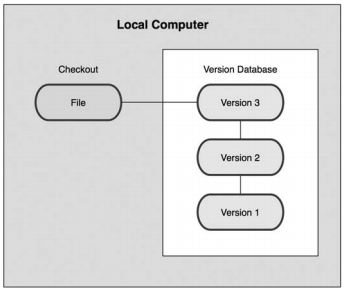
\includegraphics[width=0.4\linewidth]{Bilder/LVKS.png}
	\captionof{figure}[Lokale Architektur]{Lokale Architektur  \cite{chacon2009pro}\footnotemark }
	\label{fig:osgi}
\end{minipage}
\newpage
\subsubsection{Zentralisierte Versionskontrollsysteme}
Bei zentralisierten Versionskontrollsystemen wird die Versionierung nicht lokal vorgenommen. Die Entwickler haben einen Zentralen Punkt(Abbildung 2) , einen Server und dort befindet sich der Quellcode des Projektes in einem Reposytory, zu deutsch Lager. Der unterschied zu einfachen Lokalen Systemen ist nun Offensichtlich, man braucht zumindest ein Netzwerk, um solche Systeme zu nutzen. Ein sehr beliebtes zentralisiertes System ist Subversion. Ein weiterer Vorteil gegenüber der lokalen Versionnierung, besteht darin das gemeinsames Arbeiten an einem Projekt möglich ist und bei Verwendung eines Servers der Online erreichbar ist, kann das Arbeiten auch ohne Ortsbindung ablaufen. Doch dieser Vorteil der Ortsungebundenheit, bietet einen enormen „Single Point of Failure“, denn wenn der Server ausfällt ist man nicht in der Lage seiner Arbeit nachzugehen.


\vspace{3pt}
\begin{minipage}{\linewidth}
	\centering
	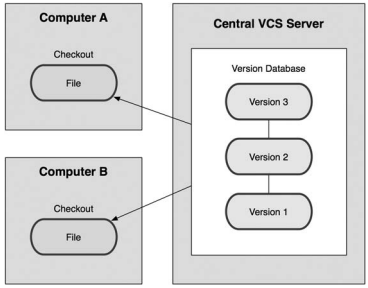
\includegraphics[width=0.3\linewidth]{Bilder/sub.png}
	\captionof{figure}[Zentralisierte Architektur]{Zentralisierte Architektur\footnotemark }
	\label{fig:osgi}
\end{minipage} 	

\subsubsection{Verteilte Versionskontrollsysteme}
GIT gehört zu den verteilten Systemen, der Unterschied zu den Varianten davor ist das sie beides können. 
Einer Art hybride Lösung, man ist in der Lage Lokal zu Versionieren aber auch im Netzwerk Versionen anderen zur Verfügung zu stellen (Abbildung 3). Jeder kann als Server fungieren und somit  wird der „Single Point of Failure“ eliminiert den zentralisierte Systeme haben. In der Praxis ist aber eher üblich, dass man einen Server nutzt vor allem bei Teamarbeiten. Wenn dieser jedoch ausfällt ist man in der Lage, weiter seine Arbeit zu verrichten.
\newline
\vspace{3pt}
\begin{minipage}{\linewidth}
	\centering
	\\textbf{includegraphics[width=0.3\linewidth]{Bilder/git.png}}
	\captionof{figure}[Verteilte Architektur]{Verteilte Architektur\footnotemark }
	\label{fig:osgi}
\end{minipage}
   

%\vspace{1em}
%\begin{minipage}{\linewidth}
%	\centering
%	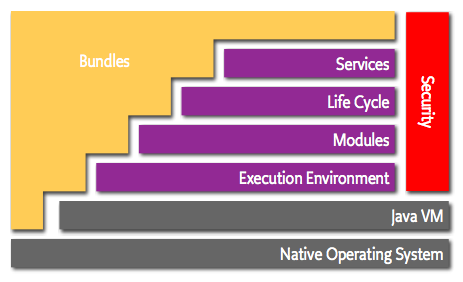
\includegraphics[width=0.7\linewidth]{Bilder/layering-osgi.png}
%	\captionof{figure}[OSGi Architektur]{OSGi Architektur\footnotemark }
%	\label{fig:osgi}
%\end{minipage}
%\footnotetext{Quelle: \url{http://www.osgi.org/Technology/WhatIsOSGi}}

\subsection{GIT Historie }
Im Jahre 2005 ist es zu Unstimmigkeiten gekommen, zwischen der Entwicklercommunity von Linux und dem Anbieter des proprietären BitKeeper-Systems, dass vorher kostenfrei genutzt wurde. Die Linux-Kernel-Entwickler mussten sich etwas einfallen lassen. Deswegen begann  Linus Torvalds im April 2005 mit der Entwicklung von GIT und präsentierte auch sehr schnell die erste Version. Git baute auf den Erfahrungen mit BitKeeper auf, doch die Hauptziele des neuen Systems waren\footnote{\cite{chacon2009pro} Seite 5}:

\begin{compactitem}
	\item Geschwindigkeit
	\item Einfaches Design
	\item Gute Unterstützung von nicht-linearer Entwicklung (tausende paralleler verschiedener Verzweigungen der Versionen)
	\item Vollständig verteilt
	\item Fähig, große Projekte wie den Linux Kernel effektiv zu verwalten
\end{compactitem}
Durch die kontinuierliche Weiterentwicklung des Systems und die Benutzerfreundlichkeit wurde Git zu einen sehr beliebten Tool.
Ein großen Einfluss auf den Erfolg von Git hat auch die Social Coding Plattform GitHub auf der man viele Open Source Projekte findet wie z.B :

\begin{compactitem}
	\item Der Linux Kernel\footnote{\cite{linux}}
	\item Ruby on Rails\footnote{\cite{ruby}}
	\item Die Javascript Bibliothek JQuery \footnote{\cite{jquery}}
	\item Das CMS Joomla\footnote{\cite{joomla}}
\end{compactitem}

Das sind natürlich nicht alle Open Source Projekte die GIT in Verbindung mit GitHub nutzen, aber einige bekannte die sich für Git entschieden haben. Der Dienst, den GitHub bereitstellt ist kostenfrei, doch nur unter der Bedingung das die Projekte öffentlich zugänglich sind. Des Weiteren gibt es Optional wählbare Services, die gegen Bezahlung verfügbar sind, aber es gibt auch eine Enterprise Version, die für Firmen interessant sein kann.    
\pagebreak

% ----------------------------------------------------------------------------------------------------------
% Kapitel
% ----------------------------------------------------------------------------------------------------------
\section{GIT Grundlagen}
Um grundlegende Funktionen von GIT zu nutzen, ist es unumgänglich gewisse Begriffe zu kennen. Elementar hingegen, ist der Umgang mit der Konsole des jeweiligen Systems. Es existieren einige plugins für Entwicklungsumgebungen, wie z.B. Eclipse die mit einem GUI ausgestattet sind. Jedoch sind diese Plugins meistens nicht soweit entwickelt, um den kompletten Funktionsumfang des Systems bedienbar zu machen,
weswegen meine Erläuterungen zum Git System, sich auf Linux als Betriebssysteme beziehen und nur mit der Konsole zu bedienen sind.     

\subsection{Begriffe die man kennen sollte}
Bevor man mit Versionierungssystemen arbeitet, sollte man einige Begriffe kennenlernen. 
\paragraph{Repository}
Der Begriff Repository (Englisch für Lager), kommt aus dem Lateinischen Repositorium.
Eine Repository ist eine spezielle Datenbank, zur systematischen Ablage von Modellen und deren Bestandteilen, das Herz der Datenhaltung eines Versionskontrollsystems. Grundlegende Funktion ist die Speicherung und das Abrufen von gespeichertem Inhalt samt aller Bestandteile wie z.B. Bilder. \footnote{\cite{Leymann}} 

\paragraph{Clone}
Ein Clone im Git Kontext, ist äquivalent zu dem begriff in der Biologie. Daher ist eine exakte Kopie von etwas existierendem, in diesem Fall der Repository. Im Fall Git lässt sich ein Clone auch durch verschiedene Protokolle umsetzten z.B. git:// ein eigens Protokoll oder auch das https:// Protokoll. Weitere Erläuterungen dazu folgen später. 
\paragraph{Commit}
Zu deutsch "übergeben", wenn man also eine Änderung im Arbeitsverzeichnis vornimmt, wird diese getrackt(verfolgt). Um diese zu bestätigen, bzw. an Git zu übergeben, ist ein commit erforderlich. 
\paragraph{Branch}
Zu Deutsch "Zweig" ist eine Gabelung des Quellcodes. Aus verschiedenen Gründen, kann es erforderlich sein eine Version des Quellcodes vom Original abzuzweigen, um ggf. eine neue Funktion zu implementieren. Dies läuft dann parallel zur Entwicklung des Originalcodes. Der initiale Commit, wird auch als Master bezeichnet 
\paragraph{Merge}
Ein Merge, bzw. das Merging ist das zusammenführen eines Branches und des Master zweiges. 



\section{Installation von GIT unter Linux}
Unter Linux ist die Installation von Git abhängig, welche Distribution genutzt wird, d.h. welches Paketmanagement-Programm. Doch es wird empfohlen wenn möglich, Git vom Quellcode aus zu installieren. Da man immer die neuste Version erhält.\footnote{\cite{chacon2009pro}} Um Git zu installieren braucht man einige Bibliotheken, die von Git verwendet werden: curl, zlib, openssl, expat und libiconv. 

Installation unter Fedora Paketmanagement (YUM)
\begin{lstlisting}
	$ yum install curl-devel expat-devel gettext-devel \openssl-devel zlib-devel
 \end{lstlisting}

Installation unter Debian/ Ubuntu
\begin{lstlisting}
	$ sudo apt-get install curl-devel expat-devel gettext-devel \openssl-devel zlib-devel
 \end{lstlisting}
 
Download GIT

\begin{lstlisting}
	http://git-scm.com/download
 \end{lstlisting}
 
 
Nachdem man diese Packete installiert hat, ist es noch notwendig Git selbst, zu downloaden. Auf dieser Seite sind Git Downloads für verschiedenste Betriebssysteme vorhanden. Um den Quellcode zu laden, wird man auf eine GitHub Repository weitergeleitet. Rechts auf dieser GitHub Page, ist immer ein Link zum Clonen, sowie ein Download link der auf dem System eine Zipdatei abspeichert. Doch um einen Überblick der verschiedenen Versionen zu bekommen 
empfehle ich den "Older releases"  link.

Anschließend wird Git kompiliert und installiert:
\begin{lstlisting}
$ tar -zxf git-2.1.3.tar.gz
$ cd git-2.1.3
$ make prefix=/usr/local all
$ sudo make prefix=/usr/local install
 \end{lstlisting}

\paragraph{Installation über den Paketmanager}

Git über den Paketmanager zu installieren, ist für Linux Anfänger durchaus praktischer. Je nach Distribution unterscheidet sich allerdings die Eingabe in das Terminal.
\newpage
Terminal Installation für Fedora/ Ubuntu/ openSUSE 

Fedora:
\begin{lstlisting}
$ yum install git
 \end{lstlisting}

Ubuntu:
\begin{lstlisting}
$ apt-get install git
 \end{lstlisting}

openSUSE :
\begin{lstlisting}
$ zypper install git
 \end{lstlisting}



\subsection{Installation unter Windows}
Auf der Homepage git-scm.com, findet man im Downloadbereich auch eine Windowsversion.
Diese wird einfach Installiert. Nach Abschluss der Installation, startet man eine seperate Git Konsole, wichtig hierbei ist, dass diese Konsole explizit nur auf Linux befehle hört. 

\subsection{Konfiguration von GIT}
Nachdem Git nun erfolgreich auf de System installiert ist, bedarf es noch einigen Konfigurationen. Über das tool \lstinline|git config| ist es möglich, durch Eingabe in das Terminal Konfigurationen vorzunehmen welche die Arbeitsweise und die Optik von Git beeinflussen. Die Konfiguratinsdateien, sind an Drei verschiedenen Orten im System
gespeichert. 
\begin{compactitem}
	\item Die Datei gitconfig im etc Verzeichniss enthält Werte, die für jeden Anwender des Systems und all ihre Projekte gelten. Durch Eingabe von\lstinline| git config| mit der Option \lstinline|--system| wird diese Datei verwendet.
\item Die Werte in der Datei \lstinline|~/.gitconfig|, gelten explizit für das Systemkonto, das gerade genutzt wird. Durch die Eingabe von\lstinline| git config| mit der Option \lstinline|--global|, wird diese Datei verwendet. 
\item Um einem Projekt, geltende Werte zuzuweisen, gibt es noch die Datei \lstinline|git/config|im Verzeichniss des Projektes selbst. 
\end{compactitem}
Wichtig ist jedoch, dass die Dateiwerte aus den jeweils vorhergehenden Dateien überschrieben wurden. Als Beispiel: \lstinline|git/config| überschreibt die Werte in \lstinline|/etc/gitconfig|

\paragraph{Konfiguration auf Windows Systemen}
Auch auf Windows sucht Git nach der \lstinline|.gitconfig| Datei im  \lstinline|$Home |Verzeichnis.  In den meisten Fällen, ist das 
der Pfad \lstinline|C:\Dokumente und Einstellungen\$USER|. Auch die \lstinline|/etc/gitconfig| Datei wird gesucht in diesem Fall, ist diese Datei in dem Verzeichnis, in das Git bei Windows installiert wurde.

\paragraph{Identität Konfigurieren}
Nachdem die Installation erfolgreich abgeschlossen wurde, ist es von enormer Wichtigkeit die Konfiguration zur Identität vorzunehmen. Git nutzt diese Parameter bei jedem Commit,
um die Einstellungen vorzunehmen das Terminal öffnen und
\begin{lstlisting}
$ git config --global user.name "Max Musterman"
$ git config --global user.email "mustermann@muster.de"
 \end{lstlisting}
Wichtig ist dabei, dass diese Einstellungen in diesem Fall nur einmal vorgenommen werden, da die Option \lstinline|--global|verwendet wird. Will man jedoch für ein explizites Projekt andere Identitätsdaten verwenden, muss man im Verzeichnis des Projekts, die selben Befehle aufrufen. Doch ohne die Option \lstinline|--global|.
\paragraph{Editor Konfiguration}
Da man beim Commiten eine Nachricht mit geben soll,  ist es möglich durch die Konsoleneingabe,  einen expliziten Texteditor zu bestimmen.
\begin{lstlisting}
$ git config --global core.editor <gewünschter Editor>
 \end{lstlisting}
Verändert man diese Einstellungsmöglichkeit jedoch nicht, wird die Default Einstellung VIM gewählt.

\paragraph{Konfiguration überprüfen}
Will man nun die vorgenommenen Einstellungen überprüfen, genügt die Eingabe dieses Befehls.
\begin{lstlisting}
$ git config --list
\end{lstlisting}

Manche der aufgelisteten Variablen, kommen vermutlich öfter vor. Dies liegt jedoch an den verschiedenen Dateien, z.B.\lstinline| /etc/gitconfig|.Iin diesem Fall wird die zuletzt aufgelistete Variable genutzt.
\newpage
\subsection{Hilfestellungen durch das System}
Für weitere spezielle Einstellungen gibt es unter Git, die Help Option.
Die gilt für fast alle Befehle, um diese auszurufen gibt es verschiedene Möglichkeiten.
\begin{lstlisting}
$ git help <verb>
$ git <verb> --help
$ man git-<verb>
\end{lstlisting} 

Braucht man nun andere Optionen zum Befehl \lstinline| git config| Tippt man folgendes in die Konsole. 
\begin{lstlisting}
$ git help config
\end{lstlisting}
Es erscheint nun ein Manual für den jeweiligen Befehl. Diese beinhaltet eine kurze Beschreibung zu der Funktion, sowie die Optionen die einem zur Verfügung stehen.  
  






\section{Mit Git Arbeiten }

Der Grundstein ist gelegt, um das Arbeiten mit Git zu beginnen. Da unser System verteilt ist, also Lokal in jedem Fall vorliegt, ist die erste Aufgabe nach erfolgreichem Installieren eine Versionierungsdatenbank zu erzeugen, ein Sogenanntes Repository. Im Allgemeinen, setzt das Arbeiten mit Git auch das Arbeiten mit der Konsole vorraus. Es besteht auch die Möglichkeit, Plugins zu nutzen die einige Funktionen unterstützen. Jedoch unterstützen diese Plugins meistens nicht alle Funktionen die Git bietet. Somit sollten die grundlegenden Konsolenbefehle bekannt sein.  
\begin{compactitem}
	\item ls - listet alle Verzeichnisse und Dateien auf, Bei Windows gilt der Befehl "dir". Mit dem Parameter -a werden auch unsichtbare Dateien angezeigt. 
	\item cd - Wechselt das Verzeichnis.
	\item cd .. - geht ein Verzeichnis zurück.
	\item mkdir - Erzeugt ein neues Verzeichnis. 
\end{compactitem}
Die Git Befehle, welche die Konsole entgegenimmt beginnen alle mit dem Signalwort GIT.  
\newpage 
\subsubsection{Ein Git Repository anlegen}
Um nun ein Repository anzulegen, navigiert man sich mit dem cd(Change Directory) Befehl in den Ordner, in welchen das Repository angelegt werden soll. Es ist aber auch Möglich ein neues Verzeichnis anzulegen mit mkdir <Name>. 

  \vspace{1em}
\begin{lstlisting}[caption=Git Repository anlegen, label=lst:arduino]
name@comp:~$ mkdir GITtest(Legt neuen Ordner an)
name@comp:~$ cd GITtest(Springt in das Verzeichnis GITtest)
name@comp:~/GITtest$ git init 
(Erzeugt ein leeres Git Repository im Ordner GITtest)
name@comp:~/GITtest$ ls -a
.  ..  .git (Erzeugntes Repository)

\end{lstlisting}

Nun ist ein Repository angelegt.
Will man nun in Zukunft ein weiteres Repository nutzen, erzeugt oder wechselt man in das Verzeichnis seiner Wahl und Tippt  \lstinline| git init| . Damit Git nun Veränderungen an Dateien tracken kann, muss man selbstverständlich diese auch in diesem Verzeichnis speichern. Doch nur das Speichern genügt Git nicht, man muss die Dateien dem Repository hinzufügen. 

 \vspace{1em}
\begin{lstlisting}[caption=Git Repository Dateien hinzufügen, label=lst:arduino]
$ git add README.txt
$ git commit -m 'initial project version'

\end{lstlisting}


Einzeln durch das Kommando \lstinline|git add DATEINAME| oder wenn es alle Dateien im Verzeichnis sind durch den Befehl \lstinline|git add -A|. Hat man seine Dateien nun hinzugefügt folgt ein Commit mit dem Kommando \lstinline|git commit-m "TEXT "|. Hat man nun alles Richtig gemacht erscheint bei der Status abfrage von git mit dem Befehl \lstinline|git status| nothing to commit (working directory clean).


\subsubsection{Ein Git Repository clonen}
Wenn im Git Kontext von Klonen die Rede ist, geht es darum ein bereits existierendes Repository, für eigene Zwecke zu Kopieren. Dies ist meist bei bereits vorhandenen Projekten der Fall. Mit \lstinline| clone [url]| wird jede einzelne Version, jeder einzelnen Datei in der Historie des Repositorys heruntergeladen. Das hat zur Folge, dass selbst wenn der Server, von dem man ursprünglich den Klone hat beschädigt wird, ist man in der Lage ihn wiederherzustellen, da der Klon alle Versionen hat. Als Beispiel ein Klon dieser Seminararbeit.

    \vspace{1em}
\begin{lstlisting}[caption=Git Repository Klonen, label=lst:arduino]
$ git clone https://github.com/veddo/FSEW.git
\end{lstlisting}

Beim diesem Vorgang legt Git ein Verzeichnis namens grit an und installiert die .git Datei darin, lädt alle Dateien des Repositorys runter und checkt die Arbeitskopie der letzten Version aus.




\subsection{ Änderungen nachverfolgen}
Man hat jetzt ein voll funktionsfähiges Git Repository und eine ausgecheckte Arbeitskopie.  Wie bereits vorher erwähnt, hat Git immer die selbe Abfolge von Kommandos, wenn man eine oder auch mehrere Dateien dem Repository hinzufügen möchte. Zur Wiederholung
\begin{compactitem}
	\item \lstinline|git status| - Überprüft den Status der Dateien im Repository.
	\item \lstinline|git add| - Lassen sich neue Dateien oder geänderte Dateien hinzufügen. 
	\item \lstinline|git commit -m "TEXT"| - Erzeugt einen snapshot aller zum Repository hinzugefügten Dateien.
\end{compactitem}
\paragraph{File Status Lifecyrcle}
Was da genau vorgeht, beschreibt am besten der File Status Lifecyrcle. Jede Datei im Arbeitsverzeichnis, kann sich in einem von zwei Zuständen befinden. Änderungen werden verfolgt (eng. Tracked) oder sie werden nicht mitverfolgt(engl. untracked). 
Genauer gesagt: Dateien welche getrackt werden sind nur die, die sich im letzten Commit befinden. Die anderen Daten die nicht, mit dem add Kommando einem Commit hinzugefügt wurden, haben den Status Untracked. \newline


\newline
\newline
\vspace{1em}
\begin{minipage}{\linewidth}
	\centering
	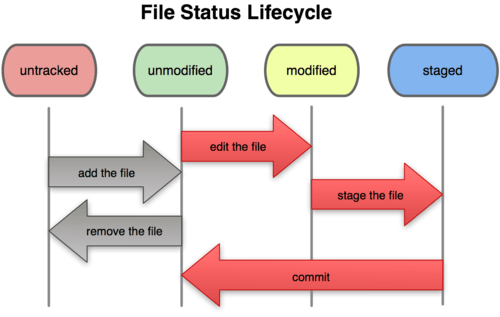
\includegraphics[width=0.6\linewidth]{Bilder/flc.png}
	\captionof{figure}[File Status Lifecycle]{Zentralisierte Architektur\footnotemark }
	\label{fig:osgi}
\end{minipage} 	

Dateien die sich nun im Commit befinden, haben wiederum zwei mögliche Stadien in denen sie sich befinden können, Veränderte (engl. modified) oder unverändert (eng. unmodified). Die veränderten Dateien sind somit für den nächsten Commit vorgemerkt (engl. staged). Alle anderen Dateien, mit dem Status unmodified werden hingegen nicht Versioniert. Sobald man nun Dateien wieder bearbeitet, beginnt dieser Vorgang erneut.

\paragraph{Zustand der Dateien Prüfen}
Der Befehl \lstinline|git status| wurde bereits weiter oben schon erwähnt und kurz erklärt, damit man eine grobe Vorstellung hat. Nun schauen wir ihn detaillierter an. Im Groben überprüft das Kommando, in welchen Status des File Life Cyrcle man sich befindet. Hat man nun ein Repository gerade geklont, bekommt man folgendes ausgegeben:

\vspace{1em}
\begin{lstlisting}[caption=Git Statusbefehl nach git clone befehl, label=lst:arduino]
$ git status
On branch master
nothing to commit, working directory clean 
\end{lstlisting}

Nach Abbildung 4 ist der momentane Status des Arbeitsverzeichnisses Unmodified, d.h. 
es wurden weder Dateien hinzugefügt, noch wurde an einer anderen Datei etwas verändert. Wenn doch, würde git die veränderten und hinzugefügten Dateien auflisten.

Fügen wir nun eine neue Datei hinzu. 
\vspace{1em}
\begin{lstlisting}[caption=Git Statusbefehl nachdem erzeugen einer Datei, label=lst:arduino]
$ touch TEST.txt
$ git status
On branch master
Untracked files:
  (use "git add <file>..." to include in what will be committed)

        TEST.txt

nothing added to commit but untracked files present (use "git add" to track)

\end{lstlisting}

Wie man an der Meldung von Git erkennen kann, gibt es Dateien, die sich im untracked status befinden. Mit der Anmerkung use \lstinline|git add| to Track, weist Git nun daraufhin, dass die neue Datei in den Status unmodified gebracht werden muss. Nach dem hinzufügen der Datei, durch \lstinline|git add[Dateiname]| und einer erneuten Statusabfrage, meldet Git folgendes:
Im File Lifecycle ist man also an erster Stelle.
\newpage
\vspace{1em}
\begin{lstlisting}[caption=Git Statusbefehl nachdem erzeugen einer Datei, label=lst:arduino]
$ git status
On branch master
Changes to be committed:
  (use "git reset HEAD <file>..." to unstage)

        new file:   TEST.TXT

\end{lstlisting}
Der Status "Changes to be committed" sagt aus, dass sich Git die neue Datei vorgemerkt (gestaged) hat und erstellt beim nächsten Commit, einen snapshot dieser Datei. Wenn man sich nun den File Status Lifecycle noch einmal anschaut, befindet man sich zwischen modified und staged. Nun bedarf es wieder dem Git add Befehl, um die Datei für den Commit vorzubereiten. Nach dem Commit hat man nun wieder eine Saubere (Clean working directory). 

\vspace{1em}
\begin{lstlisting}[caption=Git Statusbefehl nachdem verändern einer Datei, label=lst:arduino]
$ git status
On branch master
Changes to be committed:
  (use "git reset HEAD <file>..." to unstage)

      
        modified:   TEST.txt

\end{lstlisting}
Verändert man nun diese Datei, indem man einen kleinen Text hinzufügt. Sollte man wieder den Status abfragen( Listing 7 )
Dem File Status Lifecycle zufolge ist man im modified Status. 

\subsection{ Dateien ignorieren}
In den meisten Fällen kommt es vor, dass man einige Dateien gar nicht versionieren muss/soll, z.B. automatisch generierte Dateien wie Logfiles. In diesem Fall bietet Git eine Möglichkeit, dies zu Konfigurieren. Wie bei anderen Einstellungen ist es nötig, diese in einer Konfigurationsdatei zu hinterlegen, für die es klare Regeln gibt. Eine dieser festen Regeln ist der Name dieser Datei, sie muss .gitignore heißen.

Weitere Regeln im Bezug auf die .gitignore Datei sind:

\begin{compactitem}
	\item Leere Zeilen oder Zeilen, die mit # beginnen, werden 			     ignoriert.
	\item Standard glob Muster funktionieren.
	\item Man kann ein Muster mit einem Schrägstrich (/) abschließen, um ein Verzeichnis zu deklarieren.
	\item  Man kann ein Muster negieren, indem man ein Ausrufezeichen (!) voranstellt.
\end{compactitem}

Ein Beispiel für die .gitignore Datei:
\vspace{1em}
\begin{lstlisting}[caption=Git Einstellungen der.gitignore Datei, label=lst:arduino]
# ein Kommentar - dieser wird ignoriert
# ignoriert alle Dateien, die mit .a enden
*.a
# nicht aber lib.a Dateien (obwohl obige Zeile *.a ignoriert)
!lib.a
# ignoriert eine TODO Datei nur im Wurzelverzeichnis, nicht aber
/TODO
# ignoriert alle Dateien im build/ Verzeichnis
build/
# ignoriert doc/notes.txt, aber nicht doc/server/arch.txt
doc/*.txt
# ignoriert alle .txt Dateien unterhalb des doc/ Verzeichnis
doc/**/*.txt
\end{lstlisting}

Diese Datei lässt sich auch mit Hilfe der Konsole erzeugen und bearbeiten. Beim Bearbeiten helfen Editoren wie VIM oder NANO. 
\vspace{1em}
\begin{lstlisting}[caption=Git Erstellen der.gitignore Datei, label=lst:arduino]
# Erzeugt die Datei 
$ touch .gitignore
$vi .gitignore
\end{lstlisting}

Nach aufrufen des Editors, kann man nun die Dateien ausschließen, welch nicht versioniert werden sollen.
 

\subsection{Commithistorie anzeigen}
Manchmal ist es nötig einige Commits genauer einzusehen. Diese Funktion erfüllt der Befehl  \lstinline|git log|. Das Kommando listet die Historie der Commits eines Projekts, in umgekehrter chronologischer Reihenfolge auf. Des weiteren hat dieser Befehl sehr viele Optionen die man wählen kann. Eine sehr nützliche Option ist \lstinline|git log -p|, sie zeigt auf welche Änderungen gemacht wurden. Das ganze lässt sich auch eingrenzen, indem man einen weiteren Parameter hinzufügt. Als Beispiel \lstinline|git log -p -2| zeigt nur die Änderungen der letzten beiden Commits an.

\vspace{1em}
\begin{lstlisting}[caption=Git log Unterschiede der letzten 2 Commits, label=lst:arduino]
commit efb60ed05541f3bfae026c989f8b2f0cf6a2f42e
Author: Vedad Hamamdzic <vhamamdz@stud.hs-heilbronn.de>
Date:   Sun Nov 16 14:58:44 2014 +0100

    World!

diff --git a/Gittest.txt b/Gittest.txt
index 336f590..5aae200 100644
--- a/Gittest.txt
+++ b/Gittest.txt
@@ -1 +1 @@
-Hallo World
+Hallo World!

commit 04a24f7d6f2a998ec0f30ae289172e7cf07689d9
Author: Vedad Hamamdzic <vhamamdz@stud.hs-heilbronn.de>
Date:   Sun Nov 16 14:58:14 2014 +0100

    World

diff --git a/Gittest.txt b/Gittest.txt
index e69de29..336f590 100644
--- a/Gittest.txt
+++ b/Gittest.txt
@@ -0,0 +1 @@
+Hallo World
\end{lstlisting}
Da die Reihenfolge umgekehrt chronologisch aufgelistet wird, ist der letzte Commit oben zu sehen. Die beiden Commitnachrichten World ! und World, helfen beim Unterscheiden des gesuchten Commits. Man erkennt in Zeile 12 und 13, das zu Hallo World noch ein Ausrufezeichen dazu gekommen ist.
\newpage


\subsubsection{Filtern der Commit historie}
Eine Commithistorie kann vor allem bei Teamarbeit sehr groß werden, hierzu gibt es Filter Optionen die eine Suche ein wenig erleichtern können. 
 \vspace{1em}
\begin{table}[!h]
	\centering
	\begin{tabular}{|l|l|l|}
		\hline
		\textbf{Option} & \textbf{Beschreibung} \\
		\hline
		-(n)& Begrenzt die Ausgabe auf die letzten n commits\\
		\hline
		--since, --after & eigt nur Commits, die nach dem angegebenen Datum angelegt wurden.\\
		\hline
		--until, --before & Zeigt nur Commits, die vor dem angegebenen Datum angelegt wurden.\\
		\hline
		--author & Zeigt nur Commits, die von dem angegebenen Autor vorgenommen wurden.\\
		\hline
		--committer & Zeigt nur Commits, die von dem angegebenen Committer angelegt wurden.\\
		\hline
	\end{tabular}
	\caption{Befehle zum filtern der Commithistorie}
	\label{tab:Befehle}
\end{table}

Es besteht auch noch die Möglichkeit, sich die Commithistorie grafisch anzeigen zu lassen, und zwar mit dem Tcl/Tk Programm.
Dies wird in der Regel mit Git ausgeliefert und hört auf den Befehl gitk. Es ist im wesentlichen eine grafische Version von Git log und akzeptiert fast alle Filteroptionen, die Git log auch akzeptiert.

\vspace{3pt}
\begin{minipage}{\linewidth}
	\centering
	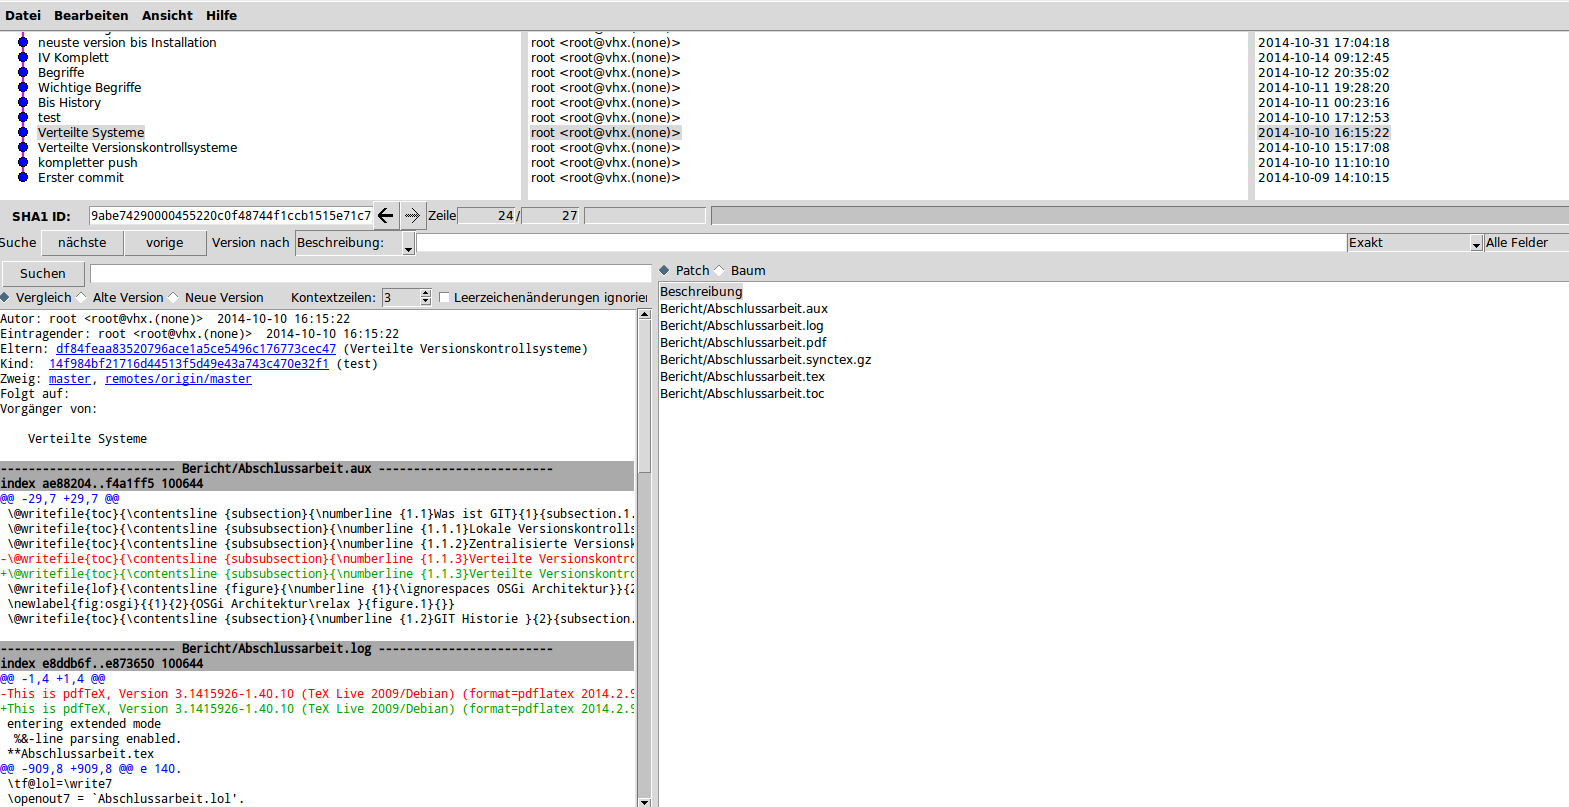
\includegraphics[width=0.9\linewidth]{Bilder/gitk.png}
	\captionof{figure}[gitk Grafische Oberfläche]{gitk Grafische Oberfläche}
	\label{fig:osgi}
\end{minipage}
Falls gitk nicht mit installiert wurde, ist es selbstverständlich nötig es zu installieren, unter Ubuntu apt-get install gitk .
Beim aufrufen sieht man die Commit Historie. Diese wird in der oberen Hälfte des Fensters dargestellt. Daneben ein Graph, der die Branches und Merges zeigt. Nach Auswahl eines Commits, zeigt die Vergleichsanzeige in der unteren Hälfte des Fensters die jeweiligen Änderungen in diesem Commit.
\newpage

%\subsection{ Änderungen rückgängig machen}
%Die Quellen befinden sich in der Datei \textit{bibo.bib}. Ein %Buch- und eine Online-Quelle sind beispielhaft eingefügt. [Vgl. %\cite{buch}, \cite{online}]

%Abkürzungen lassen sich natürlich auch nutzen (\ac{OSGi}). Weiter %oben im Latex-Code findet sich das Verzeichnis.


%Abkürzungen lassen sich natürlich auch nutzen (\ac{OSGi}). Weiter %oben im Latex-Code findet sich das Verzeichnis.
%\begin{scriptsize}
%bvc
%\end{scriptsize}
%\pagebreak

% ----------------------------------------------------------------------------------------------------------
% Kapitel 
% ----------------------------------------------------------------------------------------------------------
\section{Branching mit Git}
Lorem ipsum dolor sit amet.

\subsection{Was ist ein Branch?}
Um das Branching wirklich zu verstehen, muss man im Detail verstehen wie Git die Daten speichert.	Wenn man Commitet speichert Git	ein sogenanntes Commit-Objekt.Dieses enthält einen Zeiger zu dem Schnappschuss mit den Objekten der Staging-Area, dem Autor, den Commit-Metadaten und einem Zeiger zu den direkten Eltern des Commits. Beim Commiten bekommt jedes Projektverzeichnis eine Prüfsumme und wird  als sogenanntes tree-Objekt im Git Repository gespeichert. Sommit zeigt das Commit-Objekt auf das Tree-Objekt	diese wiederrum zeigen auf sogenannte Blops, welche den Inhalt der Dateien enthalten.	
\vspace{1em}
\begin{minipage}{\linewidth}
	\centering
	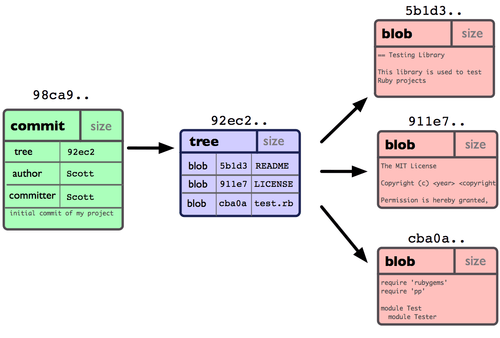
\includegraphics[width=0.6\linewidth]{Bilder/speichern.png}
	\captionof{figure}[Zentralisierte Architektur]{Speichern als Modell\footnotemark }
	\label{fig:gitspeichern}
\end{minipage} 	

Das Tree-Objekt hat die Funktion einen Inhaltsverzeichnisses im Verzeichnis jede Datei ist dort aufgelistet und  spezifiziert welcher Dateiname zu welchem Blob gehört. Des Weiteren gibt es noch einen  Zeiger, der auf die Wurzel des Projektbaumes und die Metadaten des Commits verweist (Abb.6).	 
Jede weitere Commt wird einen Zeiger enthalten, der auf den Vorhergehenden verweist. Nach zwei weiteren Commits könnte die Historie wie folgt aussehen (Abb. 7).

\vspace{1em}
\begin{minipage}{\linewidth}
	\centering
	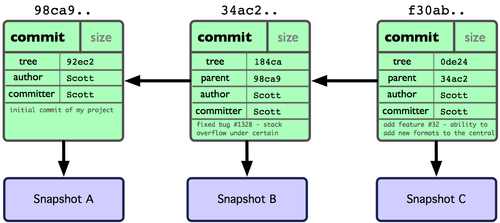
\includegraphics[width=0.6\linewidth]{Bilder/commit.png}
	\captionof{figure}[Commit Diagramm]{Speichern als Modell\footnotemark }
	\label{fig:gitspeichern}
\end{minipage} 	

Ein Branch in Git ist nichts anderes als ein simpler Zeiger auf einen dieser Commits, der Standardname eines Git-Branches lautet master. Diesen master Branch erhällt man durch den Initialen Commit der sich bei jedem neuen Commit um einz nach vorne verschiebt.
\newline
\vspace{2em}
\begin{minipage}{\linewidth}
	\centering
	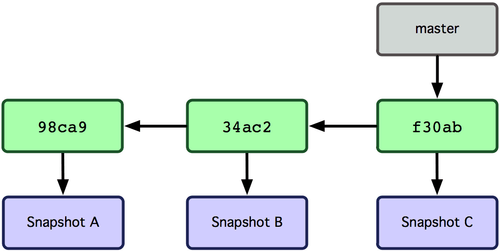
\includegraphics[width=0.6\linewidth]{Bilder/master.png}
	\captionof{figure}[Commit Diagramm]{Master Branch\footnotemark }
	\label{fig:gitspeichern}
\end{minipage} 
Wenn man nun einen neuen Branch generiert wird ein neuer Zeiger erstellt, der auf den Commit zeigt auf dem man gerade arbeitet.

\begin{lstlisting}[caption=Branch Befehl] label=lst:arduino]
$ git branch NeuerBranchName
\end{lstlisting}
\newline
\vspace{2em}
\begin{minipage}{\linewidth}
	\centering
	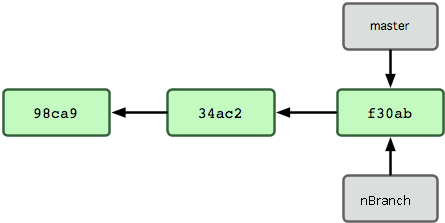
\includegraphics[width=0.6\linewidth]{Bilder/nbranch.png}
	\captionof{figure}[Commit Diagramm]{Neuer Branch\footnotemark }
	\label{fig:gitspeichern}
\end{minipage}
Nun befinden wir uns immer noch auf dem Masterzweig das bedeutet man muss in den gerade erstellten Branch wechseln.
Dies macht man mit dem Checkout Befehl.
\begin{lstlisting}[caption=Branch Befehl] label=lst:arduino]
$ git checkout 
$ git checkout NeuerBranchName
\end{lstlisting}
Um den zu sehen in welchen Branch man sich befindet kann man auf das Kommando \lstinline|git branch|zurückgreifen. Der Zweig welcher mit dem Sternchen gekennzeichnet ist, ist der indem man Arbeitet. Dieses Sternchen ist ein spezieller Zeiger der sich HEAD nennt. 
\begin{lstlisting}[caption=Aktuellen Branch prüfen] label=lst:arduino]
  master
* neuerBranch
\end{lstlisting}


	
\subsection{Einfaches Branching und Merging}
Nachdem Branching ausführlich erläutert wurde, ist Mergigng  nun an der Reihe. Merging ist das zusammenführen zweier Branches zu einem Zweig.
Das kann man am besten an einem Fallbeispiel erläutern. 
Man schreibt an einer Software, die schon eine Vorgängerversion besitzt. 
man erstellt sich einen Branch für die neue Version. 
Plötzlich wird ihnen ein Fehler gemeldet in der Alten Version. Um nun sicherzustellen das man nicht die bisherigen Änderungen ( neue Version ) und den Fix des Fehlers bereitstellt, wechselt man in den Zweig der alten version. 

\vspace{1em}
\begin{minipage}{\linewidth}
	\centering
	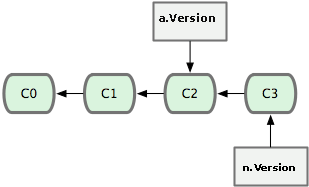
\includegraphics[width=0.6\linewidth]{Bilder/merge.png}
	\captionof{figure}[Merge]{Speichern als Modell\footnotemark }
	\label{fig:gitspeichern}
\end{minipage} 	
\newpage
Dort erstellt man sich einen weiteren Branch der als zweig aus der alten Version entsteht. Diesen kann man dann Bearbeiten und mit der alten Version mergen und ausliefern ausliefern.
 
\vspace{1em}
\begin{minipage}{\linewidth}
	\centering
	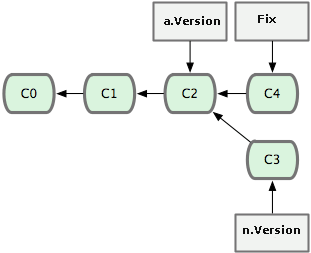
\includegraphics[width=0.6\linewidth]{Bilder/merge-fix.png}
	\captionof{figure}[Merge]{Speichern als Modell\footnotemark }
	\label{fig:gitspeichern}
\end{minipage}
Man hat nun nur die Alter Softwareversion bearbeitet ohne den neuen Code
mit in die Version zu integrieren. Durch ein einfaches checkout Kommando kann man nun wieder in seinen Zweig zurück gehen und weiter arbeiten. Jedoch sollte man auch beim mergen den File Status Lifecycle nicht außer acht lassen. denn es werden nur 2 branches gemerged die auch Commitet sind.
\pagebreak
\subsection{Merge-Konflikte}
Es kommt gelegentlich auch vor das ein Merge nicht zusammengefügt werden kann, wenn man beispielsweise an den selben stellen in Unterschiedlichen Branches was geändert hat.	
Diese Meldung über ein 'merge'-Konflikt könnte ungefähr so aussehen:
\begin{lstlisting}[caption=Branch Konfilkt] label=lst:arduino]
Auto-merging test.txt
CONFLICT (content): Merge conflict in Gittest.txt
Automatic merge failed; fix conflicts and then commit the result.
test@test:~/test$ git status
# On branch master
# Unmerged paths:
#   (use "git add/rm <file>..." as appropriate to mark resolution)
#
#	both modified:      test.txt
#
no changes added to commit (use "git add" and/or "git commit -a")


\end{lstlisting}





% ----------------------------------------------------------------------------------------------------------
% Kapitel
% ----------------------------------------------------------------------------------------------------------
\section{Merging mit Git}
Lorem ipsum dolor sit amet.

\subsection{Einfaches und Merging}
Lorem ipsum dolor sit amet, consetetur sadipscing elitr, sed diam nonumy eirmod tempor invidunt ut labore et dolore magna aliquyam erat, sed diam voluptua. At vero eos et accusam et justo duo dolores et ea rebum. Stet clita kasd gubergren, no sea takimata sanctus est Lorem ipsum dolor sit amet. Lorem ipsum dolor sit amet, consetetur sadipscing elitr, sed diam nonumy eirmod tempor invidunt ut labore et dolore magna aliquyam erat, sed diam voluptua. At vero eos et accusam et justo duo dolores et ea rebum. Stet clita kasd gubergren, no sea takimata sanctus est Lorem ipsum dolor sit amet.
\pagebreak
\section{Git in Netzwerken}
Lorem ipsum dolor sit amet, consetetur sadipscing elitr, sed diam nonumy eirmod tempor invidunt ut labore et dolore magna aliquyam erat, sed diam voluptua. At vero eos et accusam et justo duo dolores et ea rebum. Stet clita kasd gubergren, no sea takimata sanctus est Lorem ipsum dolor sit amet. Lorem ipsum dolor sit amet, consetetur sadipscing elitr, sed diam nonumy eirmod tempor invidunt ut labore et dolore magna aliquyam erat, sed diam voluptua. At vero eos et accusam et justo duo dolores et ea rebum. Stet clita kasd gubergren, no sea takimata sanctus est Lorem ipsum dolor sit amet. Semih Baby

\subsection{Welche Protokolle untersützt Git}
\pagebreak

\subsection{weg}
Zuletzt ein Beispiel für ein Listing, in dem Quellcode eingebunden werden kann, siehe Listing \ref{lst:arduino}.

\vspace{1em}
\begin{lstlisting}[caption=Arduino Beispielprogramm, label=lst:arduino]
int ledPin = 13;
void setup() {
    pinMode(ledPin, OUTPUT);
}
void loop() {
    digitalWrite(ledPin, HIGH);
    delay(500);
    digitalWrite(ledPin, LOW);
    delay(500);
}
\end{lstlisting}

In diesem Abschnitt wird eine Tabelle (siehe Tabelle \ref{tab:beispiel}) dargestellt.

\vspace{1em}
\begin{table}[!h]
	\centering
	\begin{tabular}{|l|l|l|}
		\hline
		\textbf{Name} & \textbf{Name} & \textbf{Name}\\
		\hline
		1 & 2 & 3\\
		\hline
		4 & 5 & 6\\
		\hline
		7 & 8 & 9\\
		\hline
	\end{tabular}
	\caption{Beispieltabelle}
	\label{tab:beispiel}
\end{table}



% ----------------------------------------------------------------------------------------------------------
% Literatur
% ----------------------------------------------------------------------------------------------------------
\renewcommand\refname{Quellenverzeichnis}
\bibliographystyle{myalpha}
\bibliography{bibo}
\pagebreak

% ----------------------------------------------------------------------------------------------------------
% Anhang
% ----------------------------------------------------------------------------------------------------------
\pagenumbering{Roman}
\setcounter{page}{1}
\lhead{Anhang \thesection}

\begin{appendix}
\section*{Anhang}
\phantomsection
\addcontentsline{toc}{section}{Anhang}
\addtocontents{toc}{\vspace{-0.5em}}

\section{GUI}
Ein toller Anhang.

\subsection*{Screenshot}
\label{app:screenshot}
Unterkategorie, die nicht im Inhaltsverzeichnis auftaucht.

\end{appendix}


\newpage
\thispagestyle{empty}
\begin{center}
	\vspace*{5em}
	\huge\textbf{Erklärung}\\
\end{center}
\vspace{2em}
Hiermit versichere ich, dass ich meine Abschlussarbeit selbständig verfasst und keine anderen als die angegebenen Quellen und Hilfsmittel benutzt habe.

\vspace{4em}
\begin{minipage}{\linewidth}
	\begin{tabular}{p{15em}p{15em}}
		Datum: &  .......................................................\\
		& \centering (Unterschrift)\\
	\end{tabular}
\end{minipage}

\end{document}
